\documentclass[11pt]{article}
\renewcommand{\baselinestretch}{1.5}
\setlength{\oddsidemargin}{0pt}
\setlength{\evensidemargin}{0pt}
\setlength{\topmargin}{-20pt}
\setlength{\headsep}{10pt}
\setlength{\headheight}{14pt}
\addtolength{\textheight}{1.3in}
\setlength{\textwidth}{6.2in}
\usepackage{amsmath}
\usepackage{bm}
\usepackage{amsfonts}
\usepackage{enumerate}
\usepackage{hyperref}
\usepackage{tabularx}
\usepackage{makecell}
\usepackage{graphicx}
\usepackage{authblk}
\usepackage{natbib}
\usepackage{caption}
\usepackage{subcaption}
\usepackage{algorithm}
\usepackage{float}
\usepackage{listings}
\usepackage{dsfont}
\usepackage{booktabs}
\usepackage{algorithmic}
\usepackage{multirow}
\usepackage{booktabs}
\usepackage[colorlinks=true, linkcolor=blue, urlcolor=blue]{hyperref}





\newtheorem{lemma}{Lemma}


\title{Spatiotemporal Transformer for Imputing Sparse Soil Moisture Data: A Deep Learning Approach}

\author[1]{Kehui Yao}

\affil[1]{Department of Statistics, University of Wisconsin-Madison}



\date{}

\begin{document}

\maketitle

\begin{abstract}
	Soil moisture is pivotal for environmental analyses including understanding climate dynamics and ensuring agricultural sustainability. The SMAP/Sentinel-1 soil moisture product provides a rich source of data but often comes with missing values across its spatiotemporal grid, necessitating effective imputation methods. In this paper, we introduce the Spatiotemporal Transformer model (ST-transformer) for missing values imputation in sparse spatiotemporal datasets. The model is designed with multiple spatiotemporal attention layers to capture the inherent spatiotemporal patterns. Moreover, it can seamlessly incorporate other spatiotemporal covariates during the imputation process, therefore enhancing imputation accuracy. The model training is carried out through a self-supervised approach, where the model learns to predict the missing values autonomously by leveraging observed data points. The efficacy of our model is demonstrated through its application to the SMAP 1km soil moisture data on a 36 x 36 km grid in Texas, where it shows superior accuracy over well-known imputation methods. Moreover, our simulation studies on the Healing MNIST and SMAP-HydroBlocks datasets demonstrate that our model surpasses existing state-of-the-art methods, highlighting its broader applicability in various spatiotemporal imputation tasks.	
\end{abstract}

\textbf{keywords}: Spatiotemporal Imputation, 
Transformer Model, Soil Moisture Data

\section{Introduction}
Soil moisture is essential for enhancing weather forecasts and understanding ecosystems. The NASA Soil Moisture Active Passive (SMAP) mission, launched in January 2015, aimed to provide high-resolution soil moisture data beneficial for regional or local studies. However, on July 7, 2015, the SMAP radar malfunctioned and stopped working, halting the production of high-resolution active passive soil moisture data. In the SMAP post-radar phase, various alternatives were explored to resume generating high-resolution soil moisture data. According to \citet{das2019smap}, integrating Sentinel-1A and Sentinel-1B data with SMAP radiometer data in the active-passive algorithm has the potential to retrieve soil moisture at finer spatial resolutions of 1 and 3 km. Nonetheless, a limitation arises as the temporal resolution of the SMAP active-passive data drops to a range of 3 to 12 days when utilizing Sentinel-1A and Sentinel-1B data. This reduced temporal resolution presents several challenges. Firstly, it hinders the ability to monitor and analyze short-term soil moisture dynamics, which are crucial for various applications including agriculture, drought monitoring, and flood forecasting. Secondly, the infrequent data availability can lead to inaccuracies when assessing soil moisture trends over time, potentially masking critical changes in soil conditions. Lastly, the gaps in temporal data may affect the effectiveness of real-time decision-making and resource management in response to rapidly evolving environmental conditions. 

To tackle the issue of temporal gaps in SMAP/Sentinel-1 products, imputing missing values is a common strategy. \citet{kornelsen2014comparison} examined methods including monthly average replacement (MAR), soil layer relative difference (SLRD), linear interpolation, Evolutionary Polynomial Regression (EPR), and Artificial Neural Networks (ANN) for soil moisture gap-filling. Their findings indicate that for minor data gaps (around 5\%), methods like interpolation, ANN, and EPR were comparably efficient, while MAR and SLRD were less effective. However, as the proportion of missing data increases, and gaps become larger, the effectiveness of these methods diminishes. \cite{park2023long} introduced a Multilayer Perceptron (MLP) specifically for addressing long continuous gaps rather than individual randomly missing observations. However, this approach was limited to a single time series imputation, focusing on one specific location, and did not account for spatial correlations among multiple soil moisture time series. \citet{mao2019gap} employed a two-layer machine learning-based framework to fill gaps in the SMAP/Sentinel-1 3-km product, using a model that learned mappings from various covariates to the soil moisture product, but this approach doesn't fully leverage the time series structure for gap-filling and leans more towards prediction than true imputation. This highlights a  gap in existing methodologies, where no approach integrates the rich information available in observed time series structures with supplementary covariate data for soil moisture imputation.

Moving beyond the specific area of soil moisture, the field of general time series data imputation offers a broader variety of methods. Among these, deep-learning-based imputation methods have gained attention and performed better than traditional methods in many benchmark datasets like air quality \citep{yi2016st} and healthcare \citep{silva2012predicting}, mainly because they are good at capturing complex patterns in data. 

Deep learning-based imputation methods can be broadly categorized into autoregressive methods relying on recurrent neural networks (RNNs), and non-autoregressive methods leveraging attention mechanisms. Among the autoregressive approaches, \citet{cao2018brits} proposed BRITS, which employs bidirectional recurrent neural networks for handling missing values. This method was later enhanced by \citet{cini2021filling}, who incorporated a graph neural network to better discern spatial structures. RNN-based methods possess a strong inductive bias, making them effective even on smaller datasets. However, their training process can be slow due to the sequential nature of RNNs, leading to potential error accumulation over time, especially in datasets with substantial missing values.

On the other hand, attention-based methods, introduced by \citet{vaswani2017attention}, have demonstrated remarkable performance in numerous natural language processing tasks and offer an alternative to the recurrent structure for time series imputation. For instance,\citet{du2023saits} introduced SAITS, a model using self-attention mechanisms for filling in missing values in multivariate time series. Similarly, \citet{tashiro2021csdi} proposed the idea of using a unique architecture of 2D attention (temporal attention and feature attention).  \citet{yildiz2022multivariate} introduced a transformer-based framework for multivariate time series, mainly to create pre-trained embeddings for time series, which can help with downstream filling in missing values tasks. Compared to RNNs, Transformer-based models are better at capturing long-term dependencies and understanding global context, which is crucial for accurate imputation in time series with complex relationships. Also, transformer models avoid error propagation, are easier to optimize, and have a flexible attention scope, offering a more robust framework for handling sparse observations. 


One limitation of the existing transformer-based imputation frameworks is that they primarily focus on the data needing imputation, overlooking additional contextual data. This becomes problematic, particularly in scenarios like the SMAP/Sentinel-1 product, which suffers from data sparsity. To address this, we introduce a transformer-based model that incorporates extra data sources for imputation. Specifically, our model leverages other low-resolution SMAP products and high-resolution daily ground-based observations to assist in the imputation process, with the goal of mitigating the data sparsity issue. 


Another challenge is that many existing transformer architectures are not specifically designed for spatiotemporal data. They often treat spatial information as features and use a full attention layer to learn the patterns, ignoring the common sense that nearby points are likely to be more similar, which limits its effectiveness. Additionally, when the spatial field is large, full attention doesn't scale well. To better model the spatial information, we use a shifted-window-based self-attention from \citet{liu2021swin}. The idea is to compute self-attention in non-overlapping local windows and then use a shifted window scheme to allow for connections between windows. By using a shifted window approach, we can better capture local spatial correlations, and compute more efficiently. Also, the shifted window self-attention layer is mainly used for grid data, which fits well in our context.



 We demonstrate the superior performance of our model by comparing it with other spatiotemporal imputation models, using the Texas soil moisture site data from 1 Jan 2016 to 31 Dec 2022. The model's capability is assessed by predicting the holdout SMAP/Sentinel-1 1-km soil moisture data from 1 Jan 2021 to 31 Dec 2022. Additionally, we validate the efficacy of the proposed method by comparing the imputed values with in situ measurements obtained from soil moisture networks within the study region.


The contributions of this paper are twofold. First, we present a self-supervised training framework based on a novel spatiotemporal transformer network for general spatiotemporal imputation tasks. This network is tailored to handle both the spatiotemporal response variable and spatiotemporal predicted variables concurrently. Moreover, it employs a shifted-window-based self-attention mechanism to better capture localized spatial correlations. Second, to our knowledge, this work pioneers the use of deep learning models, specifically a transformer-based model, to address missing values in the SMAP Sentinel-1 1km soil moisture data. When evaluated in the Texas study region, our model demonstrates superior performance over various time-series imputation methods by achieving the lowest mean absolute error (MAE) and mean relative error (MRE).



\section{Method}\label{sec: method}
Let $S$ represent the discrete spatial domain and $T$ represent the discrete temporal domain, with $s \in S$ and $t \in T$. Define $L=|T|$ as the total number of time points and $K=|S|$ as the total number of spatial locations. The observation at spatial location $s$ and at time $t$ is denoted as $Y(s;t)$, and the entire spatiotemporal dataset is represented as $\boldsymbol{Y} \in \mathbb{R}^{K\times L}$.
 Let $\boldsymbol{M} \in \mathbb{R}^{K \times L}$ denote a binary mask, where each element corresponds to the presence or absence of a value in $\boldsymbol{Y}$. Specifically, if the observation $Y(s;t)$ is missing, then $M(s;t) = 0$; otherwise, $M(s;t) = 1$. Let $\boldsymbol{X} \in \mathbb{R}^{K \times L \times D}$ denote the external covariates, where each element $X(s;t)$ comprises a vector of $D$ features. Furthermore, let $\tilde{\boldsymbol{Y}}$ denote the unknown complete data of $\boldsymbol{Y}$. The objective of spatiotemporal data imputation is to learn a model such that given inputs of $\boldsymbol{Y}$, $\boldsymbol{M}$, and $\boldsymbol{X}$, it yields an estimate $\hat{\boldsymbol{Y}}$ which minimizes the reconstruction error:
\begin{equation}
	L = \frac{\sum_{s=1}^K \sum_{t=1}^L l\{\hat{Y}(s;t), \tilde{Y}(s;t)\} \cdot \{1-M(s;t)\}}{\sum_{s=1}^{K}\sum_{t=1}^{L}\{1-M(s;t)\}},
\end{equation}
where $l(\cdot, \cdot)$ denotes an element-wise loss function such as mean absolute error (MAE). Given that $\tilde{\boldsymbol{Y}}$ is unknown, a surrogate objective is necessary. By randomly setting a portion of the observed values to be masked, we obtain the conditional spatiotemporal data $\boldsymbol{Y}^{o}$ and the corresponding mask $\boldsymbol{M}^{o}$. The model then attempts to reconstruct $\boldsymbol{Y}$ based on $\boldsymbol{Y}^{o}$, and the surrogate loss is evaluated on the values that have been randomly masked, expressed by:
\begin{equation}
	L = \frac{\sum_{s=1}^K \sum_{t=1}^L l\{\hat{Y}(s;t), Y(s;t)\} \cdot \{M(s;t)-M^{o}(s;t)\}}{\sum_{s=1}^{K}\sum_{t=1}^{L}\{M(s;t)-M^{o}(s;t)\}}.
	\label{eq: loss function}
\end{equation}


\subsection{Model Overview}
In this section, we present our imputation model: Spatiotemporal Transformer (ST-Transformer), as illustrated in Figure \ref{fig: st_transformer}. The model consists of three components: an input encoder, a spatiotemporal transformer encoder, and an output layer. The input encoder aggregates information at each time and location into a latent representation. The spatiotemporal transformer encoder then captures spatial and temporal dependencies within the data, enabling the model to understand underlying patterns and relationships. Finally, the output layer generates the imputed values.




\begin{figure}
\centering
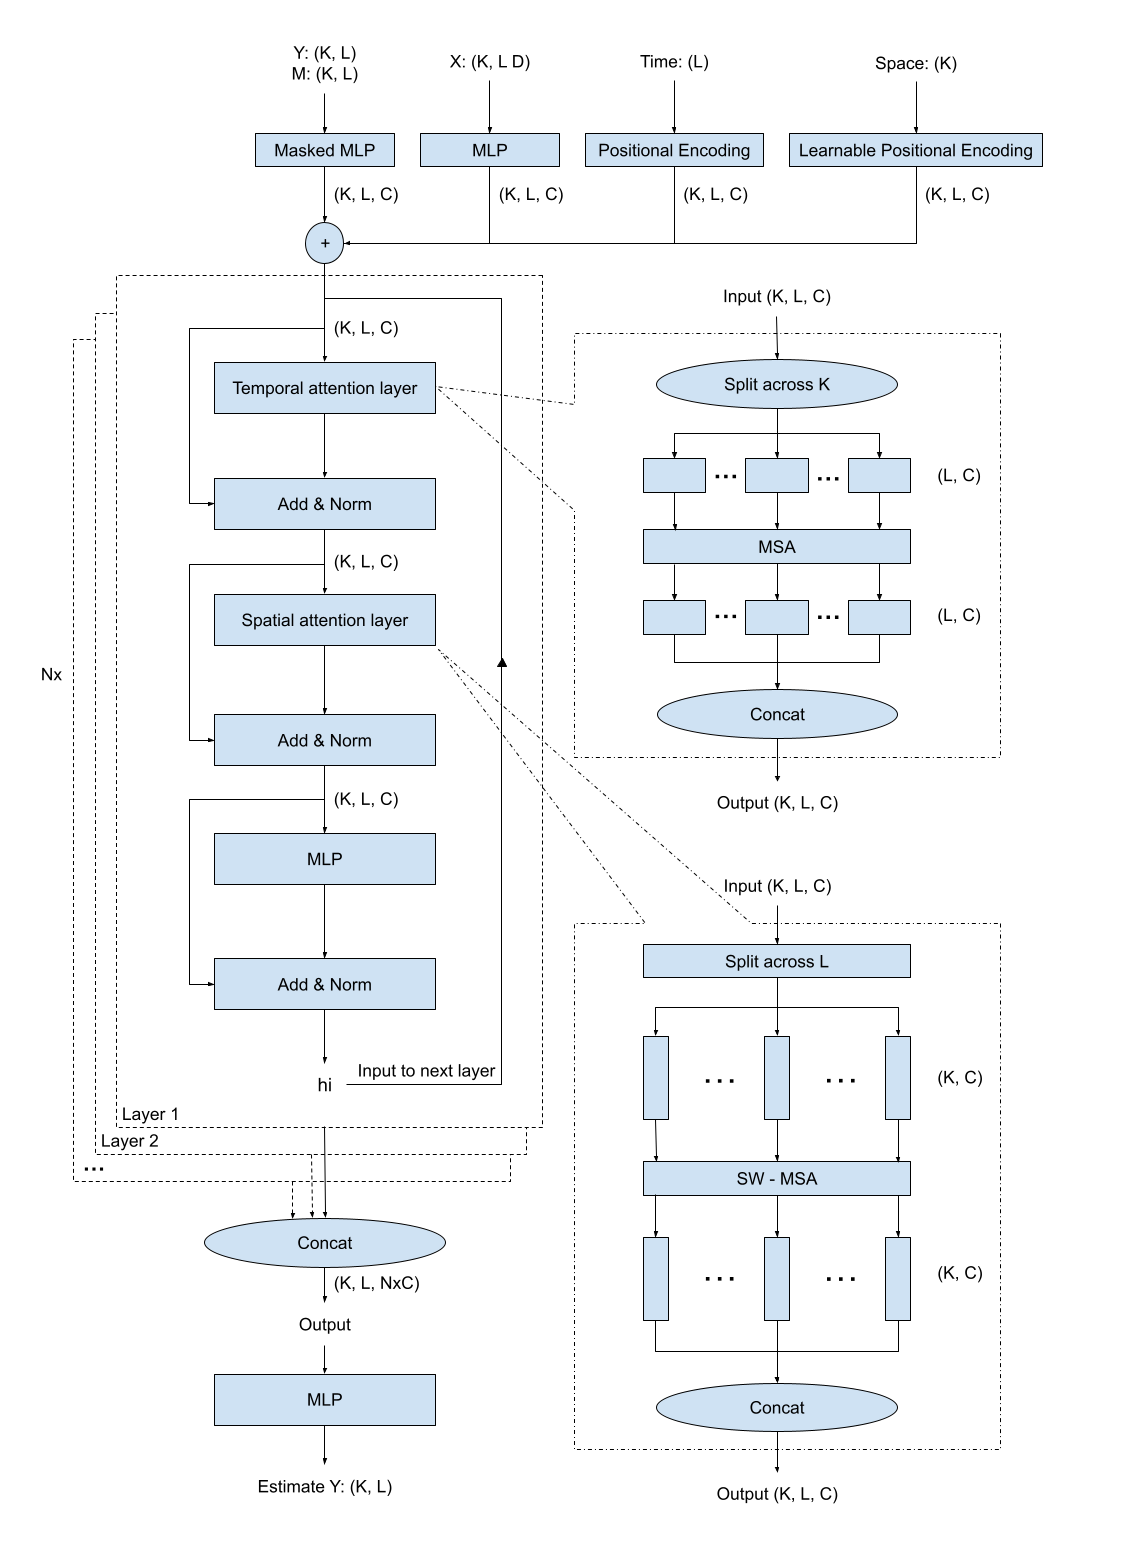
\includegraphics[width=0.8\textwidth]{figure/st_transformer.png}
\caption{The architecture of the Spatiotemporal Transformer model.}
\label{fig: st_transformer}
\end{figure}




\subsubsection*{Input Encoder} 
The input encoder consists of a Masked Multi-Layer Perceptron (MLP) to process the information from $\boldsymbol{Y}$, alongside a generic MLP for encoding the information in $\boldsymbol{X}$. It also consists of a positional encoding layer and a learnable spatial embedding layer to encode useful spatiotemporal positional information.


Mathematically, the process can be described as follows. Let $Y(s;t)$, $M(s;t)$, and $X(s;t)$ represent the observed data, missing data indicator, and predictive variables at location $s$ and time $t$ respectively. The masked MLP processes $Y(s;t)$ and $M(s;t)$ to produce an encoded representation $E_{Y}(s;t)$, formulated as: 

\begin{equation}
    E_{Y}(s;t) = \text{MLP}\{Y(s;t)\}\cdot M(s;t) + \text{mask-token} \cdot \{1-M(s;t)\},
\end{equation}
where $\text{mask-token}$ is a constant vector of dimension $C$. Similarly, the generic MLP processes $X(s;t)$ to yield an encoded representation $E_{X}(s;t)$, expressed as:
\begin{equation}
	E_{X}(s;t) = \text{MLP}(X(s;t)).
\end{equation}
The temporal position is encoded through a positional encoding layer following the approach in \citep{vaswani2017attention}. Specifically, the positional encoding for a position $t$ is given by:

\begin{align}
    E_{\text{time}2i}(t) &= \sin\left(\frac{t}{10000^{\frac{2i}{C}}}\right),\\
    E_{\text{time}2i+1}(t) &= \cos\left(\frac{t}{10000^{\frac{2i}{C}}}\right),
\end{align}

where the indices $2i$ and $2i+1$ represent the dimension indices of the positional encoding.
For spatial embedding, a learnable spatial embedding layer is used to obtain a representation $E_{\text{space}}(s)$ of the spatial location $s$:
\begin{equation}
	E_{\text{space}}(s) = \text{MLP}(s).
\end{equation}
The final unified latent representation $h(s;t)$ is then obtained by summing up these four encoded representations, as shown in the following equation:
\begin{equation}
	h(s;t) = E_{Y}(s;t) + E_{X}(s;t) + E_{\text{time}}(t) + E_{\text{space}}(s).
\end{equation}
 Therefore, $h(s;t)$ incorporates the essential spatiotemporal information along with the observed data and predictive variables.






\subsubsection*{Spatiotemporal Transformer Encoder}
The Spatiotemporal Transformer Encoder aims to encode valuable information for each data point by processing the spatial, temporal, and feature dimensions in the hidden data. It consists of multiple identical spatiotemporal attention layers, each connected via residual connections and layer normalization  \citep{ba2016layer}. Each layer comprises a temporal attention layer, a spatial attention layer, and an MLP, also linked through residual connections and layer normalization. The term "Transformer Encoder" in the model's name reflects its foundational architecture inspired by the Transformer's encoder in \citet{vaswani2017attention}. Our encoder adapts the original transformer encoder to model both spatial and temporal information. 


For the temporal attention layer, the input tensor is initially partitioned along the spatial axis, with each segment then processed through a multi-head self-attention layer (MSA) \citep{vaswani2017attention}. The processed segments are then merged to formulate the output of the temporal attention layer.


For the spatial attention layer, two variants are introduced. The first mirrors the temporal attention layer, differing only in the axis along which the input tensor is split and rejoined. However, for larger spatial dimensions, the conventional MSA encounters scalability issues. To mitigate this, the second variant adopts a stack of shifted-window-based multi-head self-attention (SW-MSA), as proposed in \citet{liu2021swin}, to replace the standard MSA to ensure efficient modeling.

Now we briefly discuss the MSA and SW-MSA. MSA allows attention across varying positions within the input sequence by projecting the input data into multiple subspaces and performing self-attention in each of these subspaces simultaneously. Mathematically, the MSA layer is formulated as follows:



\begin{equation}
    \text{MSA}(x) = \text{Concat}(\text{head}_1, \text{head}_2, \ldots, \text{head}_h)W_O,
\end{equation}
where 
\begin{equation}
	\text{head}_i = \text{Attention}(xW_{Qi}, xW_{Ki}, xW_{Vi}),
\end{equation}
and
\begin{equation}
    \text{Attention}(Q, K, V) = \text{softmax}\left(\frac{QK^T}{\sqrt{d_k}}\right) V.
\end{equation}
Here, $W_{Qi}, W_{Ki}, W_{Vi}$ and $W_O$ are learned weight matrices, $h$ is the number of heads, $d_k=d_{model}/h$, where $d_{\text{model}}$ is the dimensionality of the input and output vectors, and $\text{Concat}$ denotes the concatenation operation. Each head computes self-attention independently over different projections of the input data, thereby allowing the model to learn and attend to different patterns across different subspaces. The outputs of all heads are then concatenated and linearly transformed to obtain the final output of the MSA layer. 

One limitation of MSA is its quadratic complexity with respect to the sequence length. For large spatiotemporal datasets, the spatial dimension often spans a magnitude of $10^2$ (representing a $10\times 10$ grid) to $10^4$ (representing a $100 \times 100$ grid), making MSA unsuitable. Additionally, MSA computes global attention over the entire input sequence, potentially neglecting the localized spatial correlations inherent in geospatial data. 

SW-MSA, introduced by \citet{liu2021swin}, addresses the computational challenge by dividing the large spatial field into non-overlapping smaller windows, within which self-attention is computed independently within each window. To enable information exchange between windows, a shifted window strategy is utilized after initial window attention. This strategy re-partitions the data based on a shifted window, creating connections between previously non-overlapping windows, and computes masked attention within each window. It's common to stack multiple SW-MSA layers with different window shift sizes to capture spatial correlations at varying scales. The high-level picture of SW-MSA is illustrated in Figure \ref{fig: sw_msa}. For detailed insights, readers are encouraged to read the original paper by \citet{liu2021swin}. In summary, shifted-window-based MSA balances local and global attention and is more scalable compared to traditional MSA. Notably, in certain configurations, the SW-MSA can revert to the standard MSA. Unless specified otherwise, we default to using SW-MSA in the spatial attention layer in subsequent discussions.



\begin{figure}[H]
\centering
\includegraphics[width=0.5\textwidth]{figure/sw_msa.png}
\caption{Illustration of the shifted-window multi-head self-attention (SW-MSA) mechanism.}
\label{fig: sw_msa}
\end{figure}




Now, we demonstrate how the input tensor $\boldsymbol{h}$ traverses through a spatiotemporal attention layer as follows:



\begin{align}
		&\boldsymbol{h}_{\text{time}} = \big[\text{MSA}\{\boldsymbol{h}(1,\cdot)\}, \text{MSA}\{\boldsymbol{h}(2,\cdot)\}, \ldots, \text{MSA}\{\boldsymbol{h}(K,\cdot)\}\big]^{\prime}\\
		&\boldsymbol{h}= \text{LayerNorm}(\boldsymbol{h}+ \boldsymbol{h}_{\text{time}})\\
		&\boldsymbol{h}_{\text{space}} = \big[\text{SW-MSA}^n\{\boldsymbol{h}(\cdot, 1)\}, \text{SW-MSA}^n\{\boldsymbol{h}(\cdot, 2)\}, \ldots, \text{SW-MSA}^n\{\boldsymbol{h}(\cdot, L)\}\big]^{\prime}\\
		&\boldsymbol{h}= \text{LayerNorm}(\boldsymbol{h}+ \boldsymbol{h}_{\text{space}}).\\
		& \boldsymbol{h} = \text{LayerNorm}\{\boldsymbol{h} + \text{MLP}(\boldsymbol{h})\}\\
\end{align}

Here, $\text{SW-MSA}^n(x)$ is a stack of SW-MSA followed by residual connections and layer normalization. The mathematical representation is: 


\begin{align}
\text{SW-MSA}^n(x) = \text{LayerNorm}(&x + \text{SW-MSA}_{n}( \\
&\text{LayerNorm}(x + \text{SW-MSA}_{n-1}( \\
&\ldots \text{LayerNorm}(x + \text{SW-MSA}_{1}(x))\ldots )))),
\end{align}

where $\text{SW-MSA}_i(x)$ is the $i$-th SW-MSA layer. 

Suppose our encoder consists of $N$ identical spatiotemporal attention layers. Dnoting the operation of a single layer (as outlined in the preceding procedure) as $L(\cdot)$, and the input to the $i$-th layer as $\boldsymbol{h}_i$, the input to the $(i+1)$-th layer is given by:

\begin{equation}
    \boldsymbol{h}_{i+1} = \boldsymbol{h}_i + L(\boldsymbol{h}_i).
\end{equation}

Even though a single layer might suffice for simpler tasks, employing multiple layers could potentially improve performance. This enhancement arises as each additional layer provides the model an opportunity to learn more abstract representations of the input data. The final output from the encoder is formulated by concatenating the outputs from all spatiotemporal attention layers.

\subsubsection*{Output Layer}

The Output Layer of our model is a generic MLP, which aggregates the output from the spatiotemporal transformer encoder to produce the final imputation. Firstly, hidden representations from spatiotemporal encoder $\boldsymbol{h}_i$, are concatenated along the feature dimension, formulated as:

\begin{equation}
\boldsymbol{H} = \text{Concat}(\boldsymbol{h}_1, \boldsymbol{h}_2, \ldots, \boldsymbol{h}_N).\end{equation}
Subsequently, the concatenated representation $\boldsymbol{H}$ is processed through a generic MLP to generate the final output, expressed as:
\begin{equation}
\hat{\boldsymbol{Y}} = \text{MLP}(\boldsymbol{H}).
\end{equation}

\section{Real Data Analysis}
\subsection{Remote-Sensored and Ground-Based Datasets}

\subsubsection*{Region of Interest}

The Texas Soil Observation Network (TxSON) is a well-monitored area covering 1300 $\text{km}^2$ near Fredericksburg, Texas, in the central part of the Colorado River \citep{caldwell2019texas}. It has 40 soil moisture monitoring stations placed at distances of 3, 9, and 36 km within the Equal-Area Scalable Earth Grid. We selected a region of 36x36 km by setting the boundaries based on the furthest longitudinal and latitudinal coordinates of all the in situ sites within TxSON. This region was then split into a 36x36 grid, where each cell covers an area of about 1 km x 1 km. The choice of this region was driven by the presence of 40 in-situ soil moisture monitoring stations, which helped in the external validation of our imputation algorithm. In the following sections, we will describe the datasets used for our study, all of which were downloaded for this specific region for the time period from 2016-01-01 to 2022-12-31.

\subsubsection*{SPL3SMP}

Our initial dataset is SMAP L3 Radiometer Global Daily 36 km EASE-Grid Soil Moisture, Version 8 (SPL3SMP) \citep{o2021smap}, accessible at \url{https://nsidc.org/data/spl3smp/versions/8}. Within our study region, this Level-3 (L3) product offers a daily soil moisture estimate at a 36km spatial resolution under the cylindrical EASE-Grid 2.0 \citep{brodzik2012ease} projection. We will refer to this dataset as SMAP 36km in subsequent text.

\subsubsection*{SPL2SMAP\_S}
Our secondary dataset is SMAP/Sentinel-1 L2 Radiometer/Radar 30-Second Scene 3 km EASE-Grid Soil Moisture, Version 3 (SPL2SMAP\_S) \citep{das2019smap}. This Level-2 (L2) product provides soil moisture estimates at a 1km spatial resolution, based on the cylindrical EASE-Grid 2.0 \citep{brodzik2012ease} projection. We will refer to this dataset as SMAP 1km in subsequent text. However, the temporal coverage of this dataset is limited due to the less frequent revisit of the Sentinel-1 satellite, which has a revisit frequency of approximately 12 days. This infrequent revisit rate results in temporal gaps in the dataset, which is exactly what we aim to impute. Due to the low temporal resolution of this product, the resulting data contains around 95\% missing values.

\subsubsection*{Daily Surface Weather Data}
Our third dataset is Daymet Version 4 \citep{thornton1840daymet}. This dataset offers daily weather parameters such as precipitation, solar radiation, minimum and maximum daily temperature, and vapor pressure at 1km spatial resolution. 

\subsubsection*{Soil, Topography, and Land Cover Type Data}
\begin{enumerate}

    
\item \textbf{Soil Texture Data:} We obtain the soil texture data from the OpenLandMap datasets, which provide data at a spatial resolution of 250 meters \citep{hengl2018clay}. These datasets provide information on the fractions of clay and sand, soil organic carbon content, and bulk density. We aggregate this data to a coarser spatial resolution of 1km.


\item \textbf{Elevation Data:}  We obtain elevation data from the U.S. Geological Survey's (USGS) Shuttle Radar Topography Mission (SRTM) Global 1 arc-second dataset \citep{farr2007shuttle}, which has a spatial resolution of about 30 meters. We also aggregate this data to a 1km spatial resolution.
    
    \item \textbf{Land Cover Type Data:} We obtain land cover type data from NASA's Moderate Resolution Imaging Spectroradiometer (MODIS) instrument, specifically the MCD12Q1 dataset \citep{friedl2022modis}. This dataset provides classifications of land cover into various categories including forest, urban, and water, among others. We specifically select the 'LC\_Type1' band, which represents a particular classification scheme of land cover, to match the 1km spatial resolution of our study grid.
 \end{enumerate}
 
 

\subsubsection*{In Situ Soil Moisture Observations}
Within our study region, there are 40 soil moisture monitoring stations. These stations have been operational since 2015. The dataset includes mean hourly measurements of volumetric soil water content and temperature at depths of 5, 10, 20, and 50 cm. This in-situ data serves as an external validation source for the soil moisture data imputation.

Figure \ref{fig: eda_time_varying} displays the SMAP 1km, SMAP 36km, and daily surface weather data at a specific 1km $\times$ 1km spatial location over the period from January 1, 2016, to December 31, 2020. 

\begin{figure}[H]
\centering
\includegraphics[width=\textwidth]{figure/eda_time_varying.png}
\caption{SMAP 1km, SMAP 36km, and other daily surface weather data at a specific 1km $\times$ 1km spatial location over the period from January 1, 2016, to December 31, 2020.}
\label{fig: eda_time_varying}
\end{figure}










\subsection{Partitioning Data for Training, Validation, and Testing}
Let $S$ represent our spatial domain, which is a \(36 \times 36\) km grid, and $T$ our temporal domain, spanning from 2016/01/01 to 2022/12/31.
This configuration yields 1296 spatial locations and 2557 time points. We initially divide all the data temporally into two segments. The segment from 2016/01/01 to 2020/12/31 is allocated for training and validation, while the segment from 2021/01/01 to 2022/12/31 is reserved for out-of-sample testing.

In both segments, artificial missingness is induced in SPL2SMAP\_S to facilitate model validation.  We use two distinct approaches for setting missing data: one being "missing at time points", and the other "missing at random". In the former approach, we randomly select a proportion $p$ of time points, marking the data at all locations for these time points as missing. These points are used for validation. This approach to validation data selection aims to closely mirror the actual missingness patterns observed in real-world data, ensuring a meaningful reflection of model performance on unseen data. On the other hand, the later approach randomly selects a proportion $p$ of points and marks them as missing. This approach seeks to establish more general missing patterns in a spatiotemporal dataset. For both approaches, $p$ is set to 0.2. Figure \ref{fig: missing pattern} describes how these two approaches work.



\begin{figure}[H]
     \centering
      \begin{subfigure}[b]{0.45\textwidth}
		\centering
		\includegraphics[width=\textwidth]{figure/missing_at_time_points}
		\caption{}
		\label{fig: missing at time points}
	 \end{subfigure}
         \hfill
      \begin{subfigure}[b]{0.45\textwidth}
         \includegraphics[width=\textwidth]{figure/missing_at_random}
		 \caption{}
	\label{fig: missing at random}
     \end{subfigure}
    
     \caption{The image on the left describes the "missing at time points" approach. The image on the right describes the "missing at random" approach. In both images, white represents missing values, red represents observed data points, blue represents validation data points, and green represents imputed points.}
     \label{fig: missing pattern}
\end{figure}






\subsection{Imputation via Spatiotemporal Transformer Network}\label{sec: Imputation via Spatiotemporal Transformer Network}

\subsubsection*{Initial Setup}\label{sec: Model Training Setup}

Let $\boldsymbol{Y}_{\text{train}}$ denote the training dataset of SPL2SMAP\_S, with its corresponding missing mask represented by $\boldsymbol{M}_{\text{train}}$. The predictive variables, including SPL3SMP, Daily Surface Weather Data, Soil, Topography, and Land cover type data, are denoted by $\boldsymbol{X}_{\text{train}}$. In this setup, the total number of spatial locations is 1296, the total number of time points is 1827, and the total number of predictive variables is 15.


It's important to note that $\boldsymbol{X}_{\text{train}}$ may also contain missing values. To tackle this, we create a binary tensor $\boldsymbol{Z}_{\text{train}}$ with the same shape of $\boldsymbol{X}_{\text{train}}$, where $\boldsymbol{Z}_{\text{train}}$ pinpoints the missing positions within $\boldsymbol{X}_{\text{train}}$. Then we concatenate $\boldsymbol{X}_{\text{train}}$ and $\boldsymbol{Z}_{\text{train}}$ along the feature axis, yielding an updated version of $\boldsymbol{X}_{\text{train}}$. As a result, the number of predictive variables becomes 30.


Next, we divide the training data into multiple training samples. According to \citet{orth2012analysis}, soil moisture memory can last up to 40 days. In light of this, we partition $\boldsymbol{Y}_{\text{train}}$ along the temporal dimension using sliding windows with a fixed length of 72 and a stride of 12.  The chosen window length ensures that the model has access to a sufficient range of temporal data to capture the relevant short-term patterns in soil moisture without unnecessarily extending the memory window to periods where the relevance of data has decayed. This operation results in 152 temporal subsets, as illustrated in Figure \ref{fig: data_split}.

In determining the appropriate split size for the spatial grid, several factors were taken into consideration. Firstly, a grid size that is too small might result in the loss of crucial spatial correlations between points. Conversely, an overly large grid size, while potentially capturing spatial correlations, tends to include distant points that may not be spatially correlated, and significantly increases the computational burden. Therefore, a balanced grid size is needed. To determine a reasonable grid size, we use a variogram, a tool commonly used to quantify spatial correlations. Initially, a linear model was fitted at each location using the training data, from which the residuals were computed. Next, a sample uni-directional variogram was derived from these residuals to assess the spatial correlations. By analyzing the variogram, we identified that the variance stabilizes when the distance reaches 12 km, indicating a level where the spatial correlation between the furthest points within a grid becomes minimal.

We then further segment each of these temporal subsets along the spatial axis by subdividing the 36x36 km grid into 9 equally sized 12x12 km grids, illustrated in Figure \ref{fig: data_split}. This entire process yields a total of 1368 spatiotemporal subsets. The same procedure is replicated for $\boldsymbol{X}_{\text{train}}$ and $\boldsymbol{M}_{\text{train}}$. Consequently, we have 1368 training samples, where each sample consists of $\boldsymbol{Y}_i \in \mathbb{R}^{144\times 72}$, $\boldsymbol{X}_i \in \mathbb{R}^{144 \times 72 \times 30}$, and $\boldsymbol{M}_i \in \mathbb{R}^{144 \times 72}$. The purpose of segmentation is twofold. First, it functions as a data augmentation technique, providing more samples for model training. Second, it enhances the computational efficiency of the transformer model by mitigating the complexity associated with managing long sequences in the attention mechanism. 



\begin{figure}[H]
\centering
\includegraphics[width=0.8\textwidth]{figure/data_split.png}
\caption{ The process of segmenting training data into multiple training samples.}
\label{fig: data_split}
\end{figure}




\subsubsection*{Model Training}
For each training sample, we introduce artificial missing values to $\boldsymbol{Y}_i$ using the same two approaches as used in obtaining validation data. In the case where validation data are "missing at time points", we randomly select $p_i \in \{0.2, 0.5, 0.8\}$, and mark $p_i$ proportion of time points in $\boldsymbol{Y}_i$ as missing. Otherwise, we randomly mark $p_i$ proportion of entries in $\boldsymbol{Y}_i$ as missing. This procedure results in different positions and proportions of missingness across training samples, enabling the model to learn from a diverse set of scenarios and prevent overfitting.



\subsubsection*{Model Configuration}
In our model, $\text{MLP}$ is a feed-forward network comprising two linear transformations with a ReLU activation function in between, as expressed below:
\begin{equation}
    \text{MLP}(x)= \max (0, xW_1+b_1)W_2+b_2,
\end{equation}

Within the input encoder, both the hidden and output dimensions of the MLP are set to 64, alongside a spatial and temporal encoding dimension of 64. 

For the spatiotemporal transformer encoder, we use four spatiotemporal attention layers. Within each layer, the temporal attention layer uses a single-layer MSA with one attention head, while the spatial layer is explored in two variants: one with a single-layer MSA, and the other with two layers of SW-MSA. In the latter, the first layer uses a window size of $4\times 4$ with no shift (shift-size of 0), and the second layer uses a window size of $4 \times 4$ with a shift-size of 2. The hidden dimension of the MLP within the encoder is set to 64. 

In the output layer, we set the hidden dimension to 64 and the output dimension to 1 for the MLP. 

As for hyperparameters, we set the batch size as 16 and, the number of training epochs to 200. For optimization, We use Adam \citep{kingma2014adam} with a cosine scheduled learning rate, tapering from 0.001 down to 0.0001 over the training period.


\subsubsection*{Model Evaluation}
After model training, the model's performance is assessed through the imputation of the validation points. During evaluation, the training dataset is again divided into smaller subsets, akin to the training phase. However, unlike the training phase, no additional masks are applied to $\boldsymbol{Y}_i$ during evaluation. After obtaining imputations for all training samples, we reverse the splitting process to reconstruct $\boldsymbol{Y}_{\text{train}}$. In cases where multiple imputations are made at a specific point in the original data, we take the average. Finally, we evaluate the imputation performance using the mean absolute error (MAE) and mean relative error (MRE). Suppose $y_i$ is the ground truth of $i$th validation point, $\hat{y}_i$ is the corresponding imputed value, and $N$ is the number of validation points in total. Then MAE and MRE are defined as:


\begin{align}
		\text{MAE}=\frac{\sum_i^N |\hat{y}_i - y_i|}{N}\\
		\text{MRE}=\frac{\sum_i^N|\hat{y}_i-y_i|}{\sum_i^N|y_i|}
\end{align}


Next, we apply the same procedure to assess the model's performance on the test data. Since the test data is untouched during training, it serves as a reliable measure of the model's generalization ability.



\subsection{Comparison with Baseline Methods}
Our model is benchmarked against various simple and advanced imputation methods. These methods include:


\begin{enumerate}
	\item \textbf{Mean}: For each location, missing values are replaced with the location mean.
	\item \textbf{Linear Interpolation}: Missing values are estimated by drawing a straight line between two known values and finding the value at the missing point along this line.
	\item \textbf{Matrix Factorization}: Matrix Factorization is used to impute missing values by decomposing the original data matrix into two lower-dimensional matrices, capturing underlying patterns and structures. The missing values are then estimated by reconstructing the data matrix from these factorized matrices.
	\item \textbf{Mice}: MICE \citep{white2011multiple} works by performing multiple imputations through a series of regression models, each time estimating missing values, thus creating multiple imputed datasets. The final imputation could be an average of these datasets.
	\item \textbf{ImputeTS}:  ImputeTS \citep{moritz2017imputets} is an R package for missing value imputation, which utilizes the state space model and Kalman smoothing.
	\item \textbf{Random Forest}: Random Forest \citep{breiman2001random} utilizes an ensemble of decision trees to predict missing values, considering each missing entry as a target variable while treating others as features.
	\item \textbf{GRIN}: GRIN \citep{cini2021filling} uses a Graph-based Bidirectional Recurrent Neural Network to capture spatial and temporal dependencies in data, leveraging these relationships to impute missing values.
	\item \textbf{CSDI}: CSDI \citep{tashiro2021csdi} introduces a conditional score-based diffusion model for probabilistic imputation.
\end{enumerate}


Among the discussed methods, Mean, Linear Interpolation, Matrix Factorization, and ImputeTS do not utilize any predictive variables. In contrast, with minor modifications, the GRIN and CSDI models can incorporate covariates to assist in imputation. It's also worth noting that methods such as Mean, Matrix Factorization, MICE, and Random Forest solely rely on predictive variables to impute missing values, disregarding the inherent time series structural information. However, other methods do consider the time series information in the imputation process.

Additionally, methods such as MF and MICE do not offer a general model form for imputation, which requires retraining when applied to unseen datasets, thereby limiting their generalizability.



\subsection{Results}
\subsubsection*{Missing at Time Points}
Initially, we focus on data imputation where validation points are "missing at time points". For robustness, each imputation algorithm is independently executed five times. During each run, the selection of validation points is randomized, which may lead to variance in chosen points across runs.

The imputation results are presented in Table \ref{tab: missing at time points}. Our ST-Transformer models outperform the baseline models in both validation and testing datasets. Notably, the model using SW-MSA for spatial modeling is slightly better than the one using global attention. Furthermore, models that incorporate covariate information tend to perform better than those that do not, indicating the informative nature of these covariates in imputing 1km of soil moisture. Additionally, the deep learning-based methods outperform traditional methods and show greater robustness (as evidenced by smaller standard errors in five replicates). This enhanced performance could be due to their ability to model complex, non-linear relationships in the data, which traditional imputation methods might fail to capture. 


Figure \ref{fig: imputation_result} displays the imputation performance of the ST-Transformer (SW-MSA) at a selected location in the test dataset. Meanwhile, Figure \ref{fig: missing_at_time_points_smap} presents the imputation results across all locations over a span of 14 days.

\begin{figure}[H]
\centering
\includegraphics[width=\textwidth]{figure/smap_1km.png}
\caption{Imputation of SMAP 1km from 2021-01-01 to 2022-12-31 at one location. The land cover is grassland. Here, the green line is the imputed soil moisture, red $\times$ represents the observed points, and blue $\circ$ represents the testing points.}
\label{fig: imputation_result}
\end{figure}

\begin{figure}[H]
\centering
\includegraphics[width=\textwidth]{figure/missing_at_time_points_smap.png}
\caption{Imputation of SMAP 1km data spanning from July 21, 2021, to August 3, 2021. The top row displays the observed SMAP 1km data, where white spaces represent missing values. The bottom row illustrates the imputed soil moisture values.}
\label{fig: missing_at_time_points_smap} 
\end{figure}


\begin{table}[h!]
    \centering
    \begin{tabularx}{\textwidth}{llXX}
        \toprule
        Dataset & Method & MAE & MRE \\
        \midrule
        \multirow{10}{*}{Validation}&
        Mean & 0.0473 +/- 0.001& 31.12\% +/- 2.10\%  \\
        &Linear Interpolation & 0.0484 +/- 0.000 & 32.55\% +/- 0.32\%\\
        &Matrix Factorization & 0.0491+/- 0.003 & 43.25\% +/- 6.54\% \\
        &ImputeTS & 0.0413 +/- 0.002 & 27.63\% +/- 4.83\% \\
        &Mice & 0.0312 +/- 0.001& 27.32\% +/- 2.36\% \\
        &Random Forest &  0.0316 +/- 0.001&  27.25\% +/- 2.68\%\\
        &GRIN & 0.0287 +/- 0.000 & 16.76\% +/- 0.42\%\\
        &CSDI & 0.0283 +/- 0.000 &16.85\% +/- 0.50\%\\
        &ST-Transformer (MSA) & 0.0240 +/- 0.000 & 15.14\% +/- 0.59\%\\
        &\textbf{ST-Transformer (SW-MSA)} & 0.0223 +/- 0.000 & 14.66\% +/- 0.63\%\\
        
        \midrule
        \multirow{10}{*}{Testing}&Mean & 0.0482 +/- 0.000 & 32.24\% +/- 0.91\%  \\
        &Linear Interpolation & 0.0485 +/- 0.000& 32.59\% +/- 0.30\%\\
        &Matrix Factorization & 0.0408 +/- 0.005& 34.22\% +/- 4.64\% \\
        &ImputeTS & 0.0415 +/- 0.003 & 25.11\% +/- 3.3\% \\
        &Mice & 0.0312 +/- 0.001& 27.32\% +/- 2.27\% \\
        &Random Forest &  0.0344 +/- 0.001&  30.81\% +/- 1.86\%\\
        &GRIN & 0.0289 +/- 0.000 & 17.10\% +/- 0.49\%\\
        &CSDI & 0.0284 +/- 0.000 &17.51\% +/- 0.65\%\\
        &ST-Transformer (MSA) & 0.0247 +/- 0.001 & 16.62\% +/- 0.87\%\\

        &\textbf{ST-Transformer (SW-MSA)} & 0.0231 +/- 0.001 & 15.51\% +/- 0.91\%\\
        \bottomrule
        

    \end{tabularx}
    \caption{Imputation performance averaged over 5 independent runs. Data is "missing at time points". Models are various imputation algorithms.}
    \label{tab: missing at time points}
\end{table}






\subsubsection*{Missing at Random}
The "missing at time point" scenario is less common in spatiotemporal data. Typically, missing values in spatiotemporal data are distributed randomly across space and time. To ensure the generalizability of our method to these situations, we evaluate all imputation methods on the "missing at random" data. Similar to the earlier scenario, every imputation algorithm is run five times independently. The outcomes are presented in Table \ref{tab: missing at random}. Our ST-Transformer models continue to outperform all baseline models. Methods like Mean, Linear interpolation, ImputeTS, Mice, and Random Forest, which do not model spatial correlation, exhibit relatively stable performance. Interestingly, Matrix Factorization outperforms the covariate-based methods and even matches the performance of some deep learning methods, indicating that those non-missing spatial locations significantly help in the imputation. Moreover, our model with the SW-MSA layer for spatial modeling significantly outperforms the MSA layer for spatial modeling, showing that the SW-MSA layer is more suitable for capturing spatial correlation compared to global attention.



\begin{table}[h!]
    \centering
    \begin{tabularx}{\textwidth}{llXX}
        \toprule
        Dataset & Method & MAE & MRE \\
        \midrule
         \multirow{10}{*}{Validation}&Mean & 0.0483 +/- 0.000& 32.13\% +/- 0.85\%  \\
        &Linear Interpolation & 0.0466 +/- 0.000 & 30.98\% +/- 0.094\%\\
        &Matrix Factorization & 0.024+/- 0.000 & 19.33\% +/- 0.12\% \\
        &ImputeTS & 0.0410 +/- 0.002 & 27.12\% +/- 0.92\% \\
        &Mice & 0.0326 +/- 0.001& 27.01\% +/- 0.17\% \\
        &Random Forest &  0.0319 +/- 0.001&  26.55\% +/- 0.213\%\\
   		&GRIN &0.215 +/- 0.000 & 14.78\% +/- 0.43\%\\
        &CSDI & 0.211 +/- 0.000 & 14.01\% +/- 0.48\%\\
        &ST-Transformer (MSA) & 0.0192 +/- 0.000 & 12.76\% +/- 0.74\%\\
        &\textbf{ST-Transformer (SW-MSA)} & 0.0144 +/- 0.000 & 9.58\% +/- 0.63\%\\
        
        \midrule
        \multirow{10}{*}{Testing}&Mean & 0.0484 +/- 0.000 & 32.55\% +/- 0.00\%  \\
        &Linear Interpolation & 0.0467 +/- 0.000& 31.45\% +/- 0.00\%\\
        &Matrix Factorization & 0.0240 +/- 0.000& 19.33\% +/- 0.13\% \\
        &ImputeTS & 0.0415 +/- 0.003 & 25.11\% +/- 3.25\% \\
        &Mice & 0.0230 +/- 0.000& 19.07\% +/- 0.17\% \\
        &Random Forest &  0.0364 +/- 0.000&  32.91\% +/- 0.30\%\\
        &GRIN &0.220 +/- 0.000 & 15.31\% +/- 0.22\%\\
        &CSDI & 0.214 +/- 0.000 & 14.96\% +/- 0.51\%\\
        &ST-Transformer (MSA) & 0.0195 +/- 0.001 & 13.16\% +/- 0.40\%\\

        &\textbf{ST-Transformer (SW-MSA)} & 0.0146 +/- 0.001 & 9.80\% +/- 0.18\%\\
        
        \bottomrule

        
    \end{tabularx}
    \caption{Imputation performance averaged over 5 independent runs. Data is "missing at random'. Models are various imputation algorithms.}
    \label{tab: missing at random}
\end{table}

\subsection{Ablation Studies}

To highlight the effectiveness of spatiotemporal attention, we conduct an ablation study comparing four model variations: the complete ST-Transformer, a variant without spatial or temporal attention, one with only temporal attention, and another with only spatial attention. We evaluate these models on the validation data under both "missing at time points" and "missing at random" scenarios, with the results presented in Table \ref{tab: ablation_study_1}.In both scenarios, incorporating temporal and spatial attention significantly enhances imputation accuracy. Interestingly, while spatial attention doesn't markedly improve results in the "missing at time points" scenario, it brings substantial improvement in the "missing at random" scenario. One reason is that in the former scenario, observations are missing for all locations, leaving spatial information unexploited. Conversely, in the "missing at random" scenario, the model can directly leverage observed data from nearby locations for imputation.

\begin{table}[h!]
    \centering
    \begin{tabularx}{\textwidth}{XXXX}
        \toprule
         Scenario&Method & MAE & MRE \\
        \midrule
        \multirow{4}{*}{Missing at time points}&\textbf{ST-Transformer} & 0.0223 +/- 0.000 & 14.66\% +/- 0.63\%  \\
        &ST-Transformer (no space, no time) & 0.0301 +/- 0.000& 19.89\% +/- 0.73\%\\
        &ST-Transformer (no space) & 0.0257 +/- 0.000& 17.17\% +/- 0.62\% \\
        &ST-Transformer (no time) & 0.0262 +/- 0.000 & 17.89\% +/- 0.15\% \\
        \midrule
        \multirow{4}{*}{Missing at random}&\textbf{ST-Transformer} & 0.0144 +/- 0.000 & 9.58\% +/- 0.63\%  \\
        &ST-Transformer (no space, no time) & 0.0300 +/- 0.000& 19.80\% +/- 0.01\%\\
        &ST-Transformer (no space) & 0.0213 +/- 0.000& 14.17\% +/- 0.52\% \\
        &ST-Transformer (no time) & 0.0171 +/- 0.000 & 11.50\% +/- 0.21\% \\
        \bottomrule

    \end{tabularx}
    \caption{Imputation performance averaged over 5 independent runs. Data is "missing at time points". Models are ST-transformers with different structures.}
    \label{tab: ablation_study_1}
\end{table}


Additionally, we conduct another ablation study to show the impact of covariates on imputation. We categorize the covariates into two groups: time-varying features, which include SMAP 36km and daily surface weather data, and static features like soil characteristics, topography, and land cover type data.

We evaluate four model variations. The first model incorporates both time-varying and static covariates, the second model includes no covariates, the third model only uses time-varying features, and the fourth model solely employs static features. We assess these model variations under both missing data scenarios.

Table \ref{tab: ablation_study_2} presents the imputation performance. In the "missing at time points" scenario, we observe that including time-varying covariates significantly enhances the model performance, while incorporating static covariates also provides a slight improvement. Conversely, in the "missing at random" scenario, the inclusion of covariates doesn't contribute much to the performance. This is primarily because the model imputes missing values by exploiting spatial relations, making the additional covariate information less influential.


\begin{table}[h!]
    \centering
    \begin{tabularx}{\textwidth}{XXXX}
        \toprule
        Scenario&Method & MAE & MRE \\
        \midrule
        \multirow{4}{*}{Missing at time points}&\textbf{ST-Transformer} &  0.0223 +/- 0.000 & 14.66\% +/- 0.63\%  \\

        &ST-Transformer (no covariates) & 0.0404 +/- 0.001& 24.75\% +/- 1.51\%\\
        &ST-Transformer (time-varying) & 0.0254	 +/- 0.001& 16.17\% +/- 0.66\% \\
        &ST-Transformer (static) & 0.0385 +/- 0.001 & 22.39\% +/- 0.50\% \\
        \midrule
          \multirow{4}{*}{Missing at random}&\textbf{ST-Transformer} & 0.0144 +/- 0.000 & 9.58\% +/- 0.63\%  \\
        &ST-Transformer (no covariates) & 0.0155 +/- 0.001& 10.31\% +/- 0.38\%\\
        &ST-Transformer (time-varying) & 0.0147 +/- 0.001& 9.79\% +/- 0.11\% \\
        &ST-Transformer (static) & 0.0150 +/- 0.001 & 9.93\% +/- 0.15\% \\
        \bottomrule

        
    \end{tabularx}
    \caption{Imputation performance averaged over 5 independent runs. Data is "missing at time points". Models are ST-transformers with different covariates.}
    \label{tab: ablation_study_2}
\end{table}




%\subsection{In-situ Validation}




\section{Conclusion}
In this paper, we introduced the Spatiotemporal Transformer (ST-Transformer) model aimed at imputing missing values in sparse spatiotemporal datasets, using the SMAP/Sentinel-1 soil moisture data as a case study. Existing soil moisture gap-filling methods generally fall into two categories. The first relies solely on observed sequences, such as interpolation, and is effective primarily when data is randomly missing in small proportions. The second category, including approaches like Artificial Neural Networks (ANN), focuses on exploiting the relationships between various covariates. In this method, the imputed variable is used more as a means to understand the target variable, often not fully taking advantage of the time series structure for imputation and tending to resemble prediction more than actual imputation. Our model seeks to integrate the strengths of both categories: firstly, it employs a spatiotemporal transformer to model spatial-temporal correlations from available observations. By utilizing a Shifted Window Multihead Self Attention (SW-MSA) layer, the model is tailored to handle large spatial fields efficiently. Secondly, it incorporates both time-varying and static covariates to guide imputation in instances where data is extremely sparse, offering a more comprehensive approach to addressing missing soil moisture data. Additionally, we established a self-supervised training framework and illustrated its application in the context of imputing SMAP 1km data. In both real data analysis and simulation studies, our ST-Transformer model showed improved accuracy and computational efficiency compared to existing imputation methods. 







\section{Discussion}

\subsection{Limitations of Existing Soil Moisture Imputation Methods}

In this section, we discuss various existing methods for soil moisture gap filling and consider their limitations. \citet{kornelsen2014comparison} examined methods including monthly average replacement (MAR), soil layer relative difference (SLRD), linear interpolation, Evolutionary Polynomial Regression (EPR), and Artificial Neural Networks (ANN). Their findings indicate that for minor data gaps (around 5\%), methods like interpolation, ANN, and EPR were comparably efficient, while MAR and SLRD were less effective. However, as the proportion of missing data increases, and gaps become larger, the effectiveness of these methods diminishes. \cite{park2023long} introduced a Multilayer Perceptron (MLP) specifically for addressing long continuous gaps rather than individual randomly missing observations. However, this approach was limited to a single time series imputation, focusing on one specific location, and did not account for spatial correlations among multiple soil moisture time series. \citet{mao2019gap} employed a two-layer machine learning-based framework to fill gaps in the SMAP/Sentinel-1 3-km product, using a model that learned mappings from various covariates to the soil moisture product. In summary, existing soil moisture gap-filling methods generally fall into two categories. The first relies solely on observed sequences, such as interpolation, and is effective primarily when data is randomly missing in small proportions. The second category utilizes relationships between covariates, like ANN, where the imputed variable primarily helps in understanding the target variable. This approach often doesn't fully leverage the time series structure for gap-filling and leans more towards prediction than true imputation. Our model seeks to integrate the strengths of both categories: firstly, it employs a spatiotemporal transformer to model spatial-temporal correlations from available observations. Secondly, it incorporates covariates to guide imputation in instances where data is extremely sparse, offering a more comprehensive approach to addressing missing soil moisture data.


\subsection{Spatial variability of the Imputation}
In our study, we evaluated the imputation accuracy of different land covers by measuring the Mean Absolute Error (MAE) for various locations. Under the "missing at time points" scenario, we plot the MAE across space in Figure \ref{fig: mae_across_space}. We observed distinct variations in imputation accuracy among different land covers. Specifically, grasslands showed the best performance, followed by savannas, woody savannas, urban areas, and croplands. The poorer imputation in cropland and urban areas could be attributed to a scarcity of training data.


\begin{figure}[H]
     \centering
      \begin{subfigure}[b]{0.45\textwidth}
		\centering
		\includegraphics[width=\textwidth]{figure/eda_static}
		\caption{}
		\label{fig: missing at time points}
	 \end{subfigure}
         \hfill
      \begin{subfigure}[b]{0.45\textwidth}
         \includegraphics[width=\textwidth]{figure/error_across_space}
		 \caption{}
	\label{fig: missing at random}
     \end{subfigure}
     
    \begin{subfigure}[b]{\textwidth}
	\includegraphics[width=\textwidth]{figure/error_across_land_cover}
	\end{subfigure}
    
     \caption{Figure (a) illustrates the spatial distribution of the land cover types. Figure (b) shows the spatial variation of the MAE. Figure (c) provides box plots of the MAE across different land cover types.}
     \label{fig: mae_across_space}
\end{figure}






\subsection{Future Work}
In terms of future directions, there are several things to explore. On the application front, the ST-Transformer can be used for global soil moisture imputation at a 1km resolution. Additionally, its application could be explored across other environmental datasets characterized by various missing data scenarios. On the method front, while the SW-MSA is tailored for grid data, adapting it to accommodate more general spatial settings with irregularly spaced locations presents an interesting challenge and an area for further investigation.





\section{Simulation} 
To validate the effectiveness of our ST-Transformer model, we carried out many simulation studies. In this document, we present two key examples of these simulations, with additional studies detailed in the appendix.

we used two datasets: Healing Mnist and SMAP-Hydroblocks. The choice of Healing Mnist was to underscore our model's capability to manage intricate spatiotemporal patterns. The selection of the SMAP-Hydroblocks dataset was because it provides soil moisture data at a 1km spatial resolution and at a finer temporal resolution. This allowed us to simulate missing data patterns akin to those in the SPL2SMAP\_S dataset and then validate our imputation against actual observations.

\subsection{Healing Mnist Simulation}
Our initial focus was on the Healing MNIST dataset. This dataset comprises short sequences of moving MNIST digits that exhibit random rotational movements between frames. To simulate missing data scenarios, we introduced artificial missing values in each frame. These missing values follow two patterns: missing completely at random and missing not at random. In the latter case, white pixels in the images were more likely to become missing compared to black pixels. Each frame had an approximate missing ratio of 50\%. The dataset included 50,000 time series of digits for training and 10,000 for testing. Our model's performance was benchmarked against the GP-VAE model, currently considered state-of-the-art for this type of task. Our evaluations, as detailed in Table \ref{tab: healing_mnist}, demonstrated that the ST-Transformer model significantly outperformed the GP-VAE across both missing data scenarios, particularly in the missing not at random scenario where the improvement was substantial. Figure \ref{fig: healing_mnist} displays the imputation results in this scenario, illustrating the model's effectiveness in accurately imputing the missing digits.




\begin{table}[h!]
    \centering
    \begin{tabularx}{\textwidth}{XXX}
        \toprule
        Scenario&Method & MSE \\
        \midrule
        \multirow{2}{*}{Missing completely at random}&\textbf{ST-Transformer} & 0.0250+/-0,000   \\

        &GP-VAE& 0.036+/-0.000\\
       
        \midrule
          \multirow{2}{*}{Missing not at random}&\textbf{ST-Transformer} & 0.054+/-0.000  \\
        &GP-VAE&0.114+/-0.002\\
        \bottomrule

        
    \end{tabularx}
    \caption{Imputation performance averaged over 5 independent runs on the Healing MNIST dataset.}
    \label{tab: healing_mnist}
\end{table}








\begin{figure}[H]
\centering
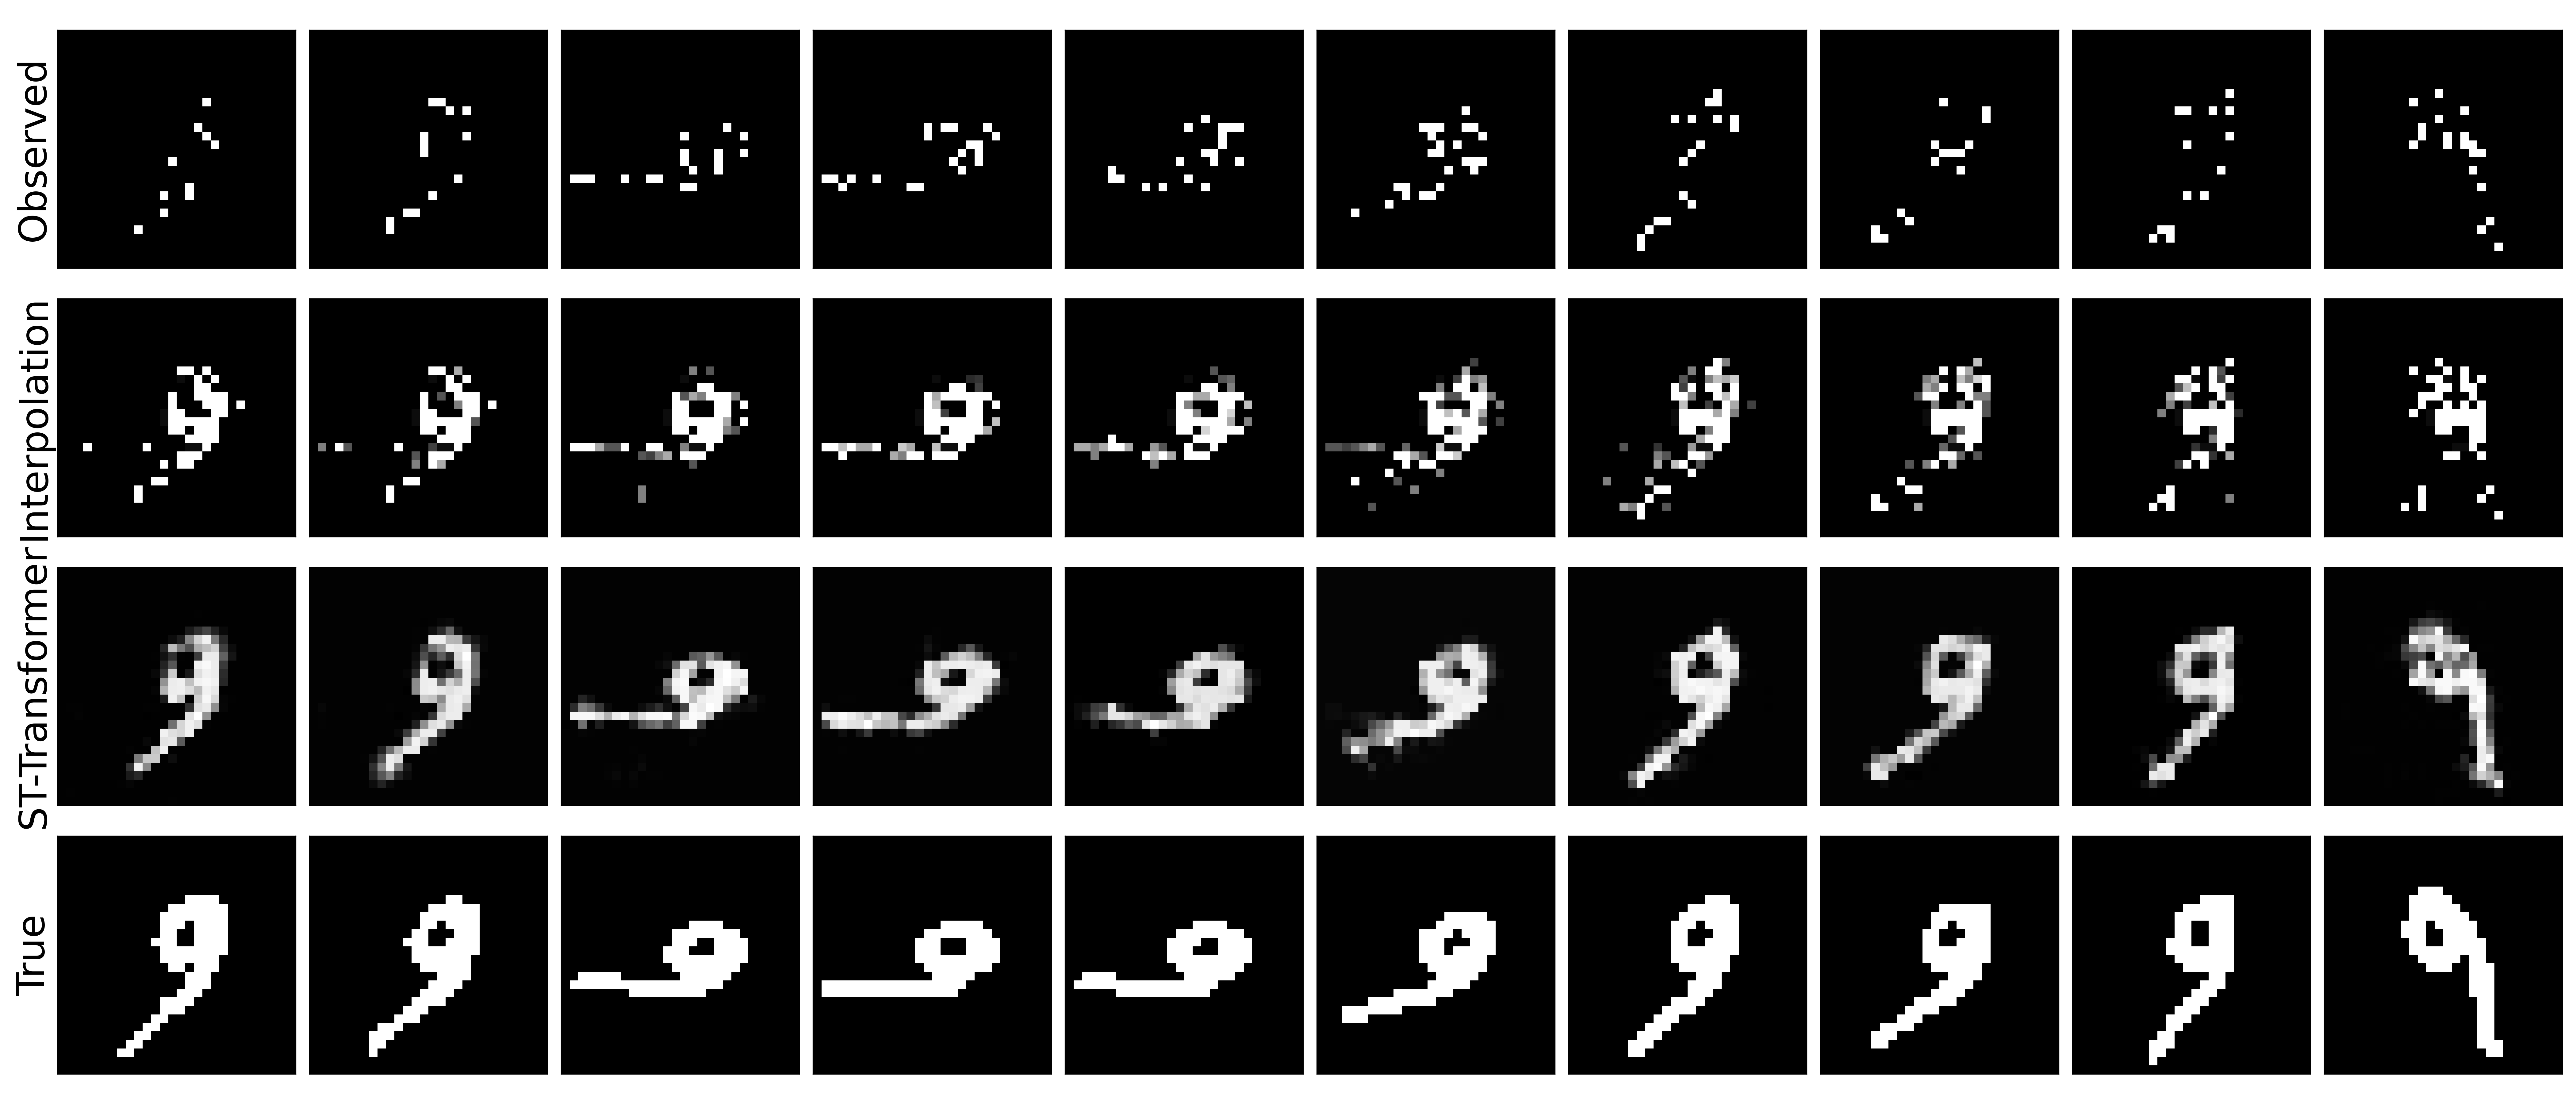
\includegraphics[width=\textwidth]{figure/healing_mnist.png}
\caption{Reconstructions from Healing MNIST. The first row displays a time series of digits with missing values. The second row shows the imputation results using the ST-Tarnsformer model. The third row shows the true sequences of the digits.}
\label{fig: healing_mnist}
\end{figure}


\subsection{SMAP-HydroBlocks}
SMAP-HydroBlocks (SMAP-HB), as detailed in \citet{vergopolan2021smap}, is a high-resolution, satellite-based surface soil moisture dataset covering the conterminous United States from 2015 to 2019 at a 30-m resolution. The dataset includes a post-processed, aggregated version at 1 km and 6-hour resolution, available at \href{https://zenodo.org/records/5206725}{https://zenodo.org/records/5206725}. To ensure consistency with our real data analysis, we extract data from a 36 $\times$ 36 km grid within the study region and incorporate covariates to help in the imputation process. We replicate the missing patterns found in the original SPL2SMAP\_S dataset and use only the observed data for imputation. Our findings, detailed in Table \ref{tab: smap_hydroblock}, indicate that the ST-Transformer continues to lead in performance compared to other models. The imputation results are visually demonstrated in Figure \ref{fig: smap_hydroblock}, highlighting the efficacy of our approach in this context.

\begin{table}[h!]
    \centering
    \begin{tabularx}{\textwidth}{lXX}
        \toprule
       Method & MAE & MRE \\
        \midrule
        Mean & 0.0456 +/- 0.002& 28.34\% +/- 0.41\%  \\
        Linear Interpolation & 0.0415 +/- 0.001 & 25.16\% +/- 0.080\%\\
        Matrix Factorization & 0.0483+/- 0.000 & 35.29\% +/- 1.36\% \\
        ImputeTS & 0.0410 +/- 0.002 & 27.12\% +/- 0.92\% \\
        Mice & 0.0286 +/- 0.001& 20.09\% +/- 0.60\% \\
        Random Forest &  0.0294 +/- 0.001&  20.35\% +/- 0.397\%\\
   		GRIN &0.259 +/- 0.000 & 16.11\% +/- 0.43\%\\
        CSDI & 0.264 +/- 0.000 & 16.50\% +/- 0.48\%\\
        ST-Transformer (MSA) & 0.024 +/- 0.000 & 15.29\% +/- 0.43\%\\
        \textbf{ST-Transformer (SW-MSA)} & 0.021 +/- 0.000 & 13.17\% +/- 0.24\%\\
        
        \bottomrule

        
    \end{tabularx}
    \caption{Imputation performance averaged over 5 independent runs. Data is SMAP HydroBlocks missing at time points. Models are various imputation algorithms.}
    \label{tab: smap_hydroblock}
\end{table}


 
\begin{figure}[H]
\centering
\includegraphics[width=\textwidth]{figure/smap_hydroblocks.png}
\caption{Imputation of SMAP 1km from 2016-01-01 to 2019-12-31 at one location using ST-Transformer. The land cover is grassland. Here, the green line is the imputed soil moisture, red $\times$ represents the observed points, and blue $\circ$ represents the testing points.}
\label{fig: smap_hydroblock}
\end{figure}
 
 
 
 
%\subsubsection*{Descriptive Spatio-Temporal Statistical Models}
%
%We assume that the true process can be expressed by spatiotemporal fixed effects attributed to covariates plus a random process varying across space and time. We then simulate the data by specifying the dependence structure in this random process. Let $S=\{1, \ldots, 36\}$ and $T=\{1, \ldots, 400\}$. So $K=36$, $L=400$. Let
%
%
%\begin{align}
%	    &Y(s;t) = Z(s;t)+\epsilon(s;t)\\
%        &Z(s;t) = f(s;t) + \eta(s;t), \\
%        &f(s;t) = X(s;t)\boldsymbol{\beta}, \\
%        &\epsilon(s;t) \sim N(0,0.1)\\
%        &\eta(s;t) \sim GP[0, C\{(s_1;t_1), (s_2;t_2)\}]\\
%        &C\{(s_1;t_1), (s_2;t_2)\} = C_s(s_1,s_2) \times C_t(t_1,t_2)\\
%        &C_s(s_1, s_2) = \exp[-0.5 \times \{(s_1-s_2)^2 / \sigma_s\}^2]\\
%        &C_t(t_1, t_2) = \exp[-0.5 \times \{(t_1-t_2) / \sigma_t\}^2]\\
%        &X(s;t) \sim \mathcal{N}(0, I_d)  
%\end{align}
%
%Here, $Y(s;t)$ is the observed spatiotemporal data, $Z(s;t)$ is the latent spatiotemporal process, and $\epsilon(s;t)$ is the spatiotemporal random error. $f(s,t)$ is the space-time fixed effect parameterized by a $d$-dimensional vector $\beta$, $X(s;t)$ are $d$-dimensional covariates simulated from a standard multivariate normal distribution. $\eta(s,t)$ is a spatiotemporal random effect following a Gaussian process with a separable spatiotemporal covariance matrix.
%
%\subsubsection*{Dynamic Spatio-Temporal Model}
%Next, we use a dynamic model instead of a descriptive model to better understand and predict changes in spatial fields over time. We simulate our data using a linear Markovian spatiotemporal process model. Following the previous definitions, our model is defined as:
%
%
%\begin{align}
%        Z(s;t) &= \sum_{x=1}^{K}m(x;s;\boldsymbol{\theta})Z(x;t-1) + \eta(s;t), \\
%        m(x;s;\boldsymbol{\theta}) &= \theta_1 \exp\{-\frac{1}{\theta_2}(x-\theta_3-s)^2\},\\
%        Y(s;t) &= Z(s;t)+\epsilon(s;t).
%\end{align}
%
%
%Here, \(Z(s;t)\) is the spatial process we're modeling. The function \(m(x;s;\boldsymbol{\theta})\) calculates how different spatial points from the previous time contribute to the current observation. The terms \(\eta(s;t)\) and \(\epsilon(s;t)\) are consistent with their earlier definitions. We set the parameters as \(\theta_1=0.2\), \(\theta_2=5\), and \(\theta_3=0\).
%
%\subsection{Missing Patterns}
%In our simulation data, we artificially introduce missing values to evaluate the performance of our models. The initial data, $\boldsymbol{Y}$, does not contain any missing values. We employ two strategies for introducing missingness. 
%
%First, we randomly mask values in $\boldsymbol{Y}$. Each observation, $Y(s;t)$, has a probability $p$ of being masked. This strategy introduces missing values scattered randomly across the data. Second, we introduce missingness in a more structured way, emulating the patterns seen in our real data. In this strategy, either all values at a specific time point are observed, or none are observed. We assign a probability $p$ to the event of all values at a time point being masked. 
%
%For both strategies, we explore different levels of missingness by using masking probabilities $p$ of 0.2, 0.5, and 0.9.


\bibliographystyle{apalike}
\bibliography{refs}



\end{document}